\chapter{Result}\label{cha:Research}
%

% Ska följa som ett naturligt komplement till huvuddelen

In this chapter, the results are presented, so that in the next chapter, these results are analysed.

%\section{Example}\label{sec:research:history}
%
Liksom \citep{Duck:2005} har vi kommit fram till att glass smakar bäst på sommaren \citep{Khalil02NonlinearSystemsBook}.

\marginpar{Kommer att tänka på en liten anekdot\ldots}

\Warning[TODO]{Ta bort den löjliga anekdoten!}

\begin{figure}[tbp]
  \centering
  \subfloat[Alldeles för tidigt.][\label{fig:times:very-early}Det här är väl tidigt — din glass hinner smälta innan ditt sällskap dyker upp.]{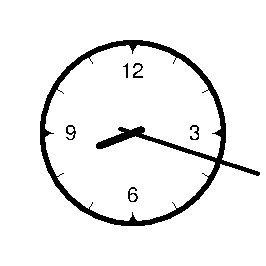
\includegraphics[page=1]{clocks}}
  \qquad
  \subfloat[Med marginal.][\label{fig:times:early}Kiosken stänger snart, men inte nu — perfekt!]{\includegraphics[page=2]{clocks}}
  \\
  \subfloat[I grevens tid.][\label{fig:times:on-time}Precis i tid — du får in ett finger i luckan just när kiosken ska stänga.  Han som jobbar blir sur, och det blir smolk i bägaren.]{\includegraphics[page=3]{clocks}}
  \qquad
  \subfloat[Försent.][\label{fig:times:late}Du är sen — kiosken är stängd.]{\includegraphics[page=4]{clocks}}
  \caption{\label{fig:times}%
    Illustration av \emph{subfloats}.  Den så kallade \emph{bounding box}en visas i \protect\subref{fig:times:late}.  Lägg märke till att bounding boxen har satts så att alla bilder har samma storlek, med enhetlig placering av själva innehållet i förhållande till bounding boxen.  Antag att du ska träffa en kompis för att äta glass just när kiosken stänger för dagen vid 08:30.  När dyker du upp?}
\end{figure}

\section{Final App Result}

\todo{Show images of final app - on mobile, tablet and desktop?}

\section{Qualitative Data from Final App Evaluation}

1. Why are they correct and incorrect?
2. Do they like it?
3. Are they stimulated by it?
4. What did they like?
5. What didn't they like?
6. When do you want to use the app?
7. When are you not able to use the app?

Three groups:

1

\section{Quantative Data from Final App Evaluation}

%\begin{chapter-appendix}

%\section{Proof-Appendix}
%
Det här är en appendix-del av det aktuella kapitlet.

%\end{chapter-appendix}
